\subsection{Topología ferroviaria original}

\lipsum[2]


\begin{figure}[H]
	\centering
	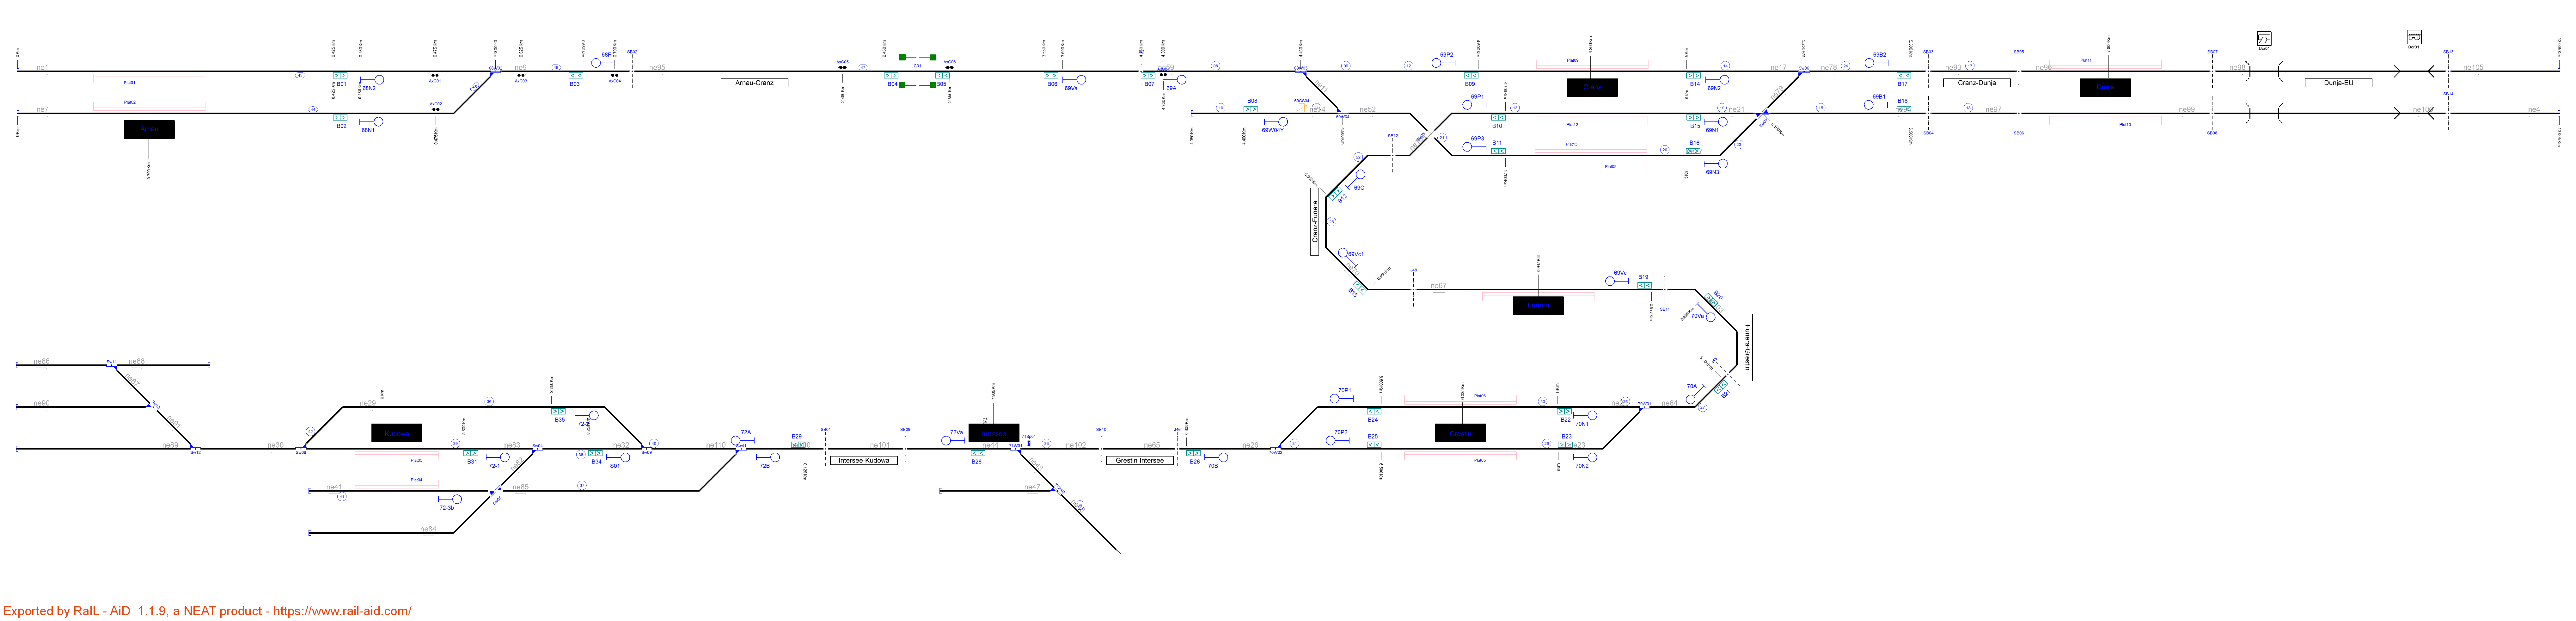
\includegraphics[width=1\textwidth]{resultados-obtenidos/ejemplo3/images/3_original.png}
	\centering\caption{Señalamiento original del ejemplo 3.}
	%\label{fig:LC_P2}
\end{figure}

\lipsum[2]

\begin{figure}[H]
	\centering
	
\includegraphics[width=1\textwidth]{resultados-obtenidos/ejemplo3/images/3_empty.png}
	\centering\caption{Topología ferroviaria del ejemplo 3 sin señalamiento.}
	%\label{fig:LC_P2}
\end{figure}

\lipsum[2]
